%! Author = Philipp Emmenegger
%! Date = 09/07/2021

\section{Introduction SPA}
\subsection{Browser-based Applications}
\textbf{Benefits}
\begin{itemize}
    \item Work from anywhere, anytime
    \item Platform independent, including mobile
    \item No software update, no application, easy maintenance
    \item Software can be provided as a service (SaaS - pay as you go)
    \item Code separation
\end{itemize}
\textbf{Liabilities}
\begin{itemize}
    \item No data sovereignty (Datenhoheit)
    \item Limited/restricted hardware access
    \item SEO - Search engines must execute JavaScript
    \item More complex deployment strategies
\end{itemize}

\subsection{SPA}
A website that fits on a single web page with a user experience similar to that of a desktop application.
All code is retrieved with a single page load or resources are dynamically loaded.
SPAs use AJAX and HTML5 to create responsive Web apps, without constant page reloads.

\subsubsection{Architecture}
Website interacts with user by rewriting parts of the DOM.
After first load, all interaction with the server happens through AJAX.
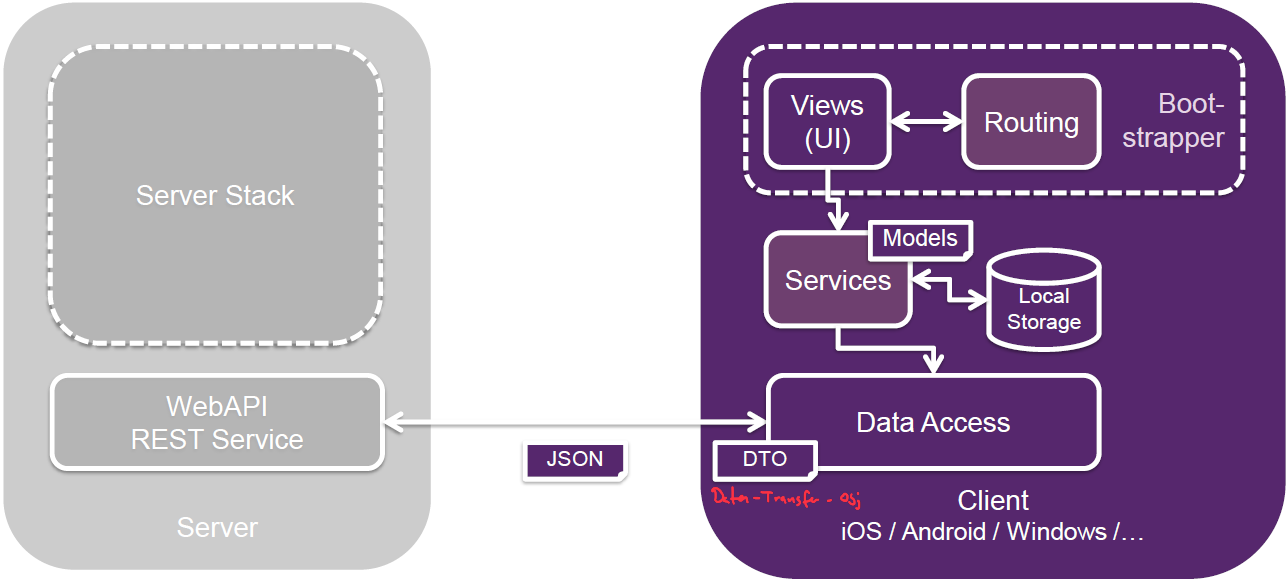
\includegraphics[width=\linewidth]{img/spa_architecture.png}

\subsubsection{Bundling}
All JS code must be delivered to the client over potentially slow networks.
Bundling and minifying the source leads to smaller SPA footprint.
Larger SPAs with many modules need a reliable dependency management.
Initial Footprint can be reduced by loading dependent modules on-demand.

\subsubsection{WebPack as Bundler}
\textbf{Entry:} Start, follows the graph of dependencies to know what to bundle.\\
\textbf{Output:} Tell webpack where to bundle your application.\\
\textbf{Loaders:} Transforms these files into modules as they are added to your dependency graph.\\
\textbf{Plugins:} Perform tasks like bundle optimization, asset management and injection of env variables.\\
\textbf{Mode:} Enable built-in optimization mechanisms.

\subsection{Routing}
\begin{itemize}
    \item Completely on client-side by JS
    \item Navigation behaves as usual
    \item Browser needs to fake the URL to change and store page state
    \item \textit{window.history.pushState}
\end{itemize}

\subsection{Dependency Injection}
\textbf{Benefits}
\begin{itemize}
    \item Reduces coupling between consumer and implementation
    \item Contracts between classes are based on interfaces
    \item Supports the open/closed principle
    \item Allows flexible replacement of an implementation
\end{itemize}

\subsubsection{Decorators}
\begin{itemize}
    \item Provide a way to add annotations / meta-programming syntax
    \item Can be attached to a class declaration, method, accessor, property or parameter
    \item Widely used in Angular
\end{itemize}